\subsection{Within-CHIME width--frequency test for unmodelled sub-components}
\label{sec:chime-subband}

A scattering index measured from a single band is only as trustworthy as the temporal model
underneath it: an unmodelled second component broadens the fitted profile and biases the recovered
$\alpha$ high. Before quoting a CHIME-side scattering index we therefore run a model-free check
\emph{within} the CHIME band. We split each burst's CHIME band ($0.40$--$0.80\,\mathrm{GHz}$) into
four $80\,\mathrm{MHz}$ sub-bands and, in each, measure two model-free widths of the
baseline-subtracted on-pulse profile: the rms width $w_{\mathrm{rms}}$ and the trailing-edge
$e$-folding time $w_{\mathrm{tail}}$. Genuine scattering predicts both widths growing toward lower
frequency as $\nu^{-\alpha}$; frequency-independent intrinsic (multi-peak) morphology does not.

\begin{figure}
\centering
% vector source is chime_subband_compare.svg; \includesvg needs the `svg' package + inkscape.
% \includegraphics finds chime_subband_compare.pdf (vector) under pdflatex without extra packages.
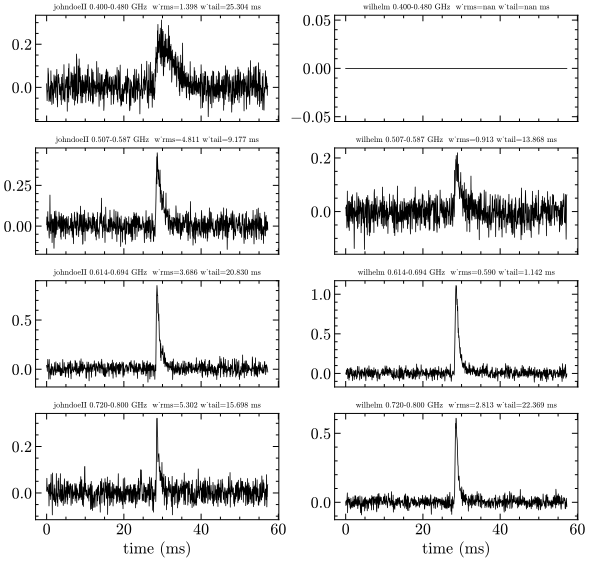
\includegraphics[width=\columnwidth]{chime_subband_compare}
\caption{Within-CHIME sub-band profiles for the co-detected FRBs johndoeII and wilhelm, each split
into four $80\,\mathrm{MHz}$ sub-bands across $0.40$--$0.80\,\mathrm{GHz}$. Each panel shows the
baseline-subtracted on-pulse profile against time, annotated with the model-free rms width
$w_{\mathrm{rms}}$ and the trailing-edge $e$-folding time $w_{\mathrm{tail}}$. A purely scattering
origin predicts both widths increasing toward lower frequency as $\nu^{-\alpha}$, whereas
frequency-independent intrinsic sub-structure does not; the empty $0.40$--$0.48\,\mathrm{GHz}$
sub-band for wilhelm is a data gap, not a non-detection. This profile-shape evolution is the
diagnostic we use to flag unmodelled temporal sub-components before a scattering index is quoted,
since such components otherwise bias the recovered $\alpha$ high.}
\label{fig:chime-subband-compare}
\end{figure}
